\subsection{Gridmap}
A grid map is a representation of the possible location of the agent in a discrete space. On the initial map generated for the agents, starting and finishing points of each agent will be indicated. A map will also include an indication of unreachable spots, which will be referred to as "walls" or "obstacles". Two possible map standards will be implemented: space-separated map and JSON-based map. The space-separated map is meant for creating and storing persistent maps, as it is also human-readable. The JSON-based map is mostly meant for machine-to-machine communication, as it is easily parsable. Conversion between those maps, as well as storage, will happen in the map service. It will be also served to the agents from this microservice, which will have the possibility of generating random maps and spawning agents on it.

Before executing an algorithm, the map will have to be translated to a graph, where each tile of the grid map represents one node of the graph. Edges of the graph represent possible agent movement. Two possible modes will be available: with and without diagonal movement\ref{fig:map_2D}. As a default algorithms will use mode without diagonal moves.

\begin{figure}[H]
    \centering
    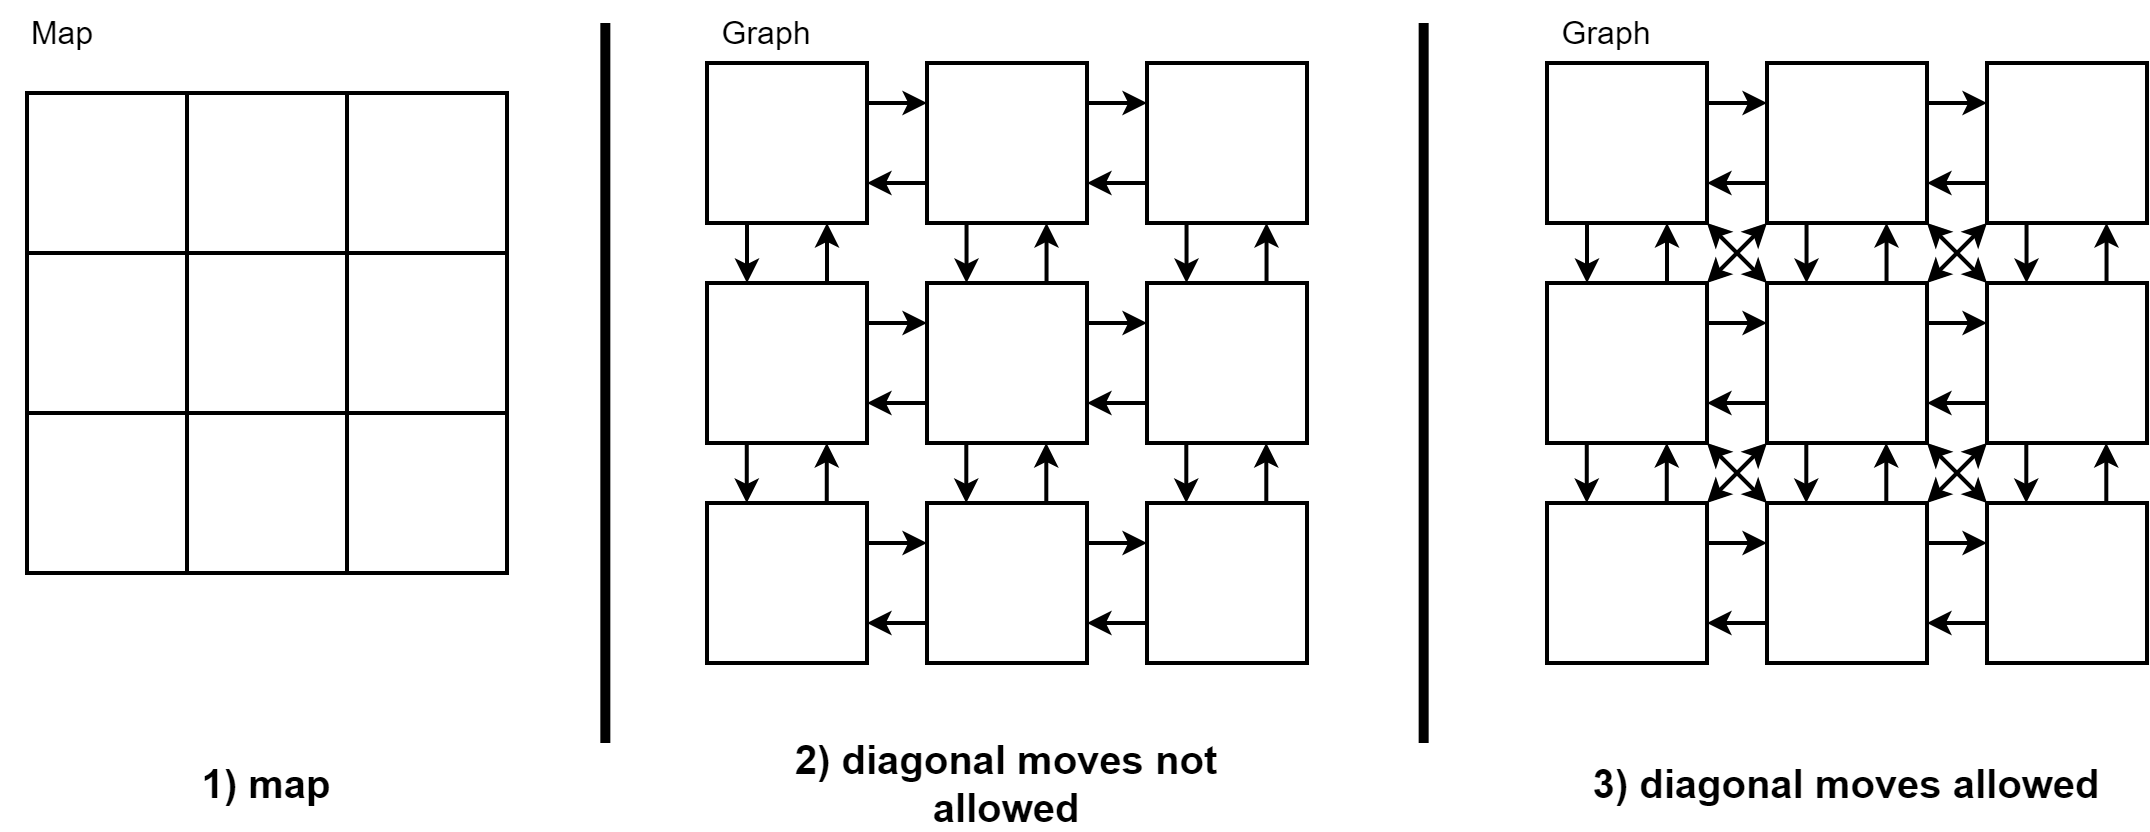
\includegraphics[width=\textwidth]{pictures/map_2d.png}
    \caption{ 2D map to graph translation }
    \label{fig:map_2D}
\end{figure}

Each tile represents the node and it is connected with two edges to neighboring tiles, which represents the possibility of two-way movement from and to neighboring tiles. 


\subsection{Gridmap for CA* algorithm}
For CA* algorithm map has to be translated into a 3d grid map where every layer is a representation of the possible location of the agent in a particular time frame and therefore time becomes the third dimension in a graph. Similar to in a 2d grid map there are two possible modes which are represented in the figure below. An agent can only move in one direction vertically as each level corresponds to one moment in time. Other tiles on each level are connected in the same way as in figure \ref{fig:map_2D}.
\begin{figure}[H]
    \centering
    \includegraphics[width=\textwidth]{pictures/map_3D.png}
    \caption{ 3D map to graph translation }
    \label{fig:map_3D}
\end{figure}
After the path is planned for specific agents, it has to be marked as an obstacle so agents which are planning their paths, later on, would be aware of unreachable/occupied tiles.

\subsection{CA* front collision problem}
Planning multiple agents' paths on a single map leads to a problem when agents are colliding with each other because they are moving in the opposite direction on the same column or row. This situation is shown in figure \ref{fig:head_collision}. Both agents assume that the tile in front of them is not occupied, which is a valid assumption. However, as this is a discrete model, a collision occurs between timeframes. To mitigate this problem, after the path is planned edges in the opposite direction of agent movement need to be removed.
\begin{figure}[H]
    \centering
    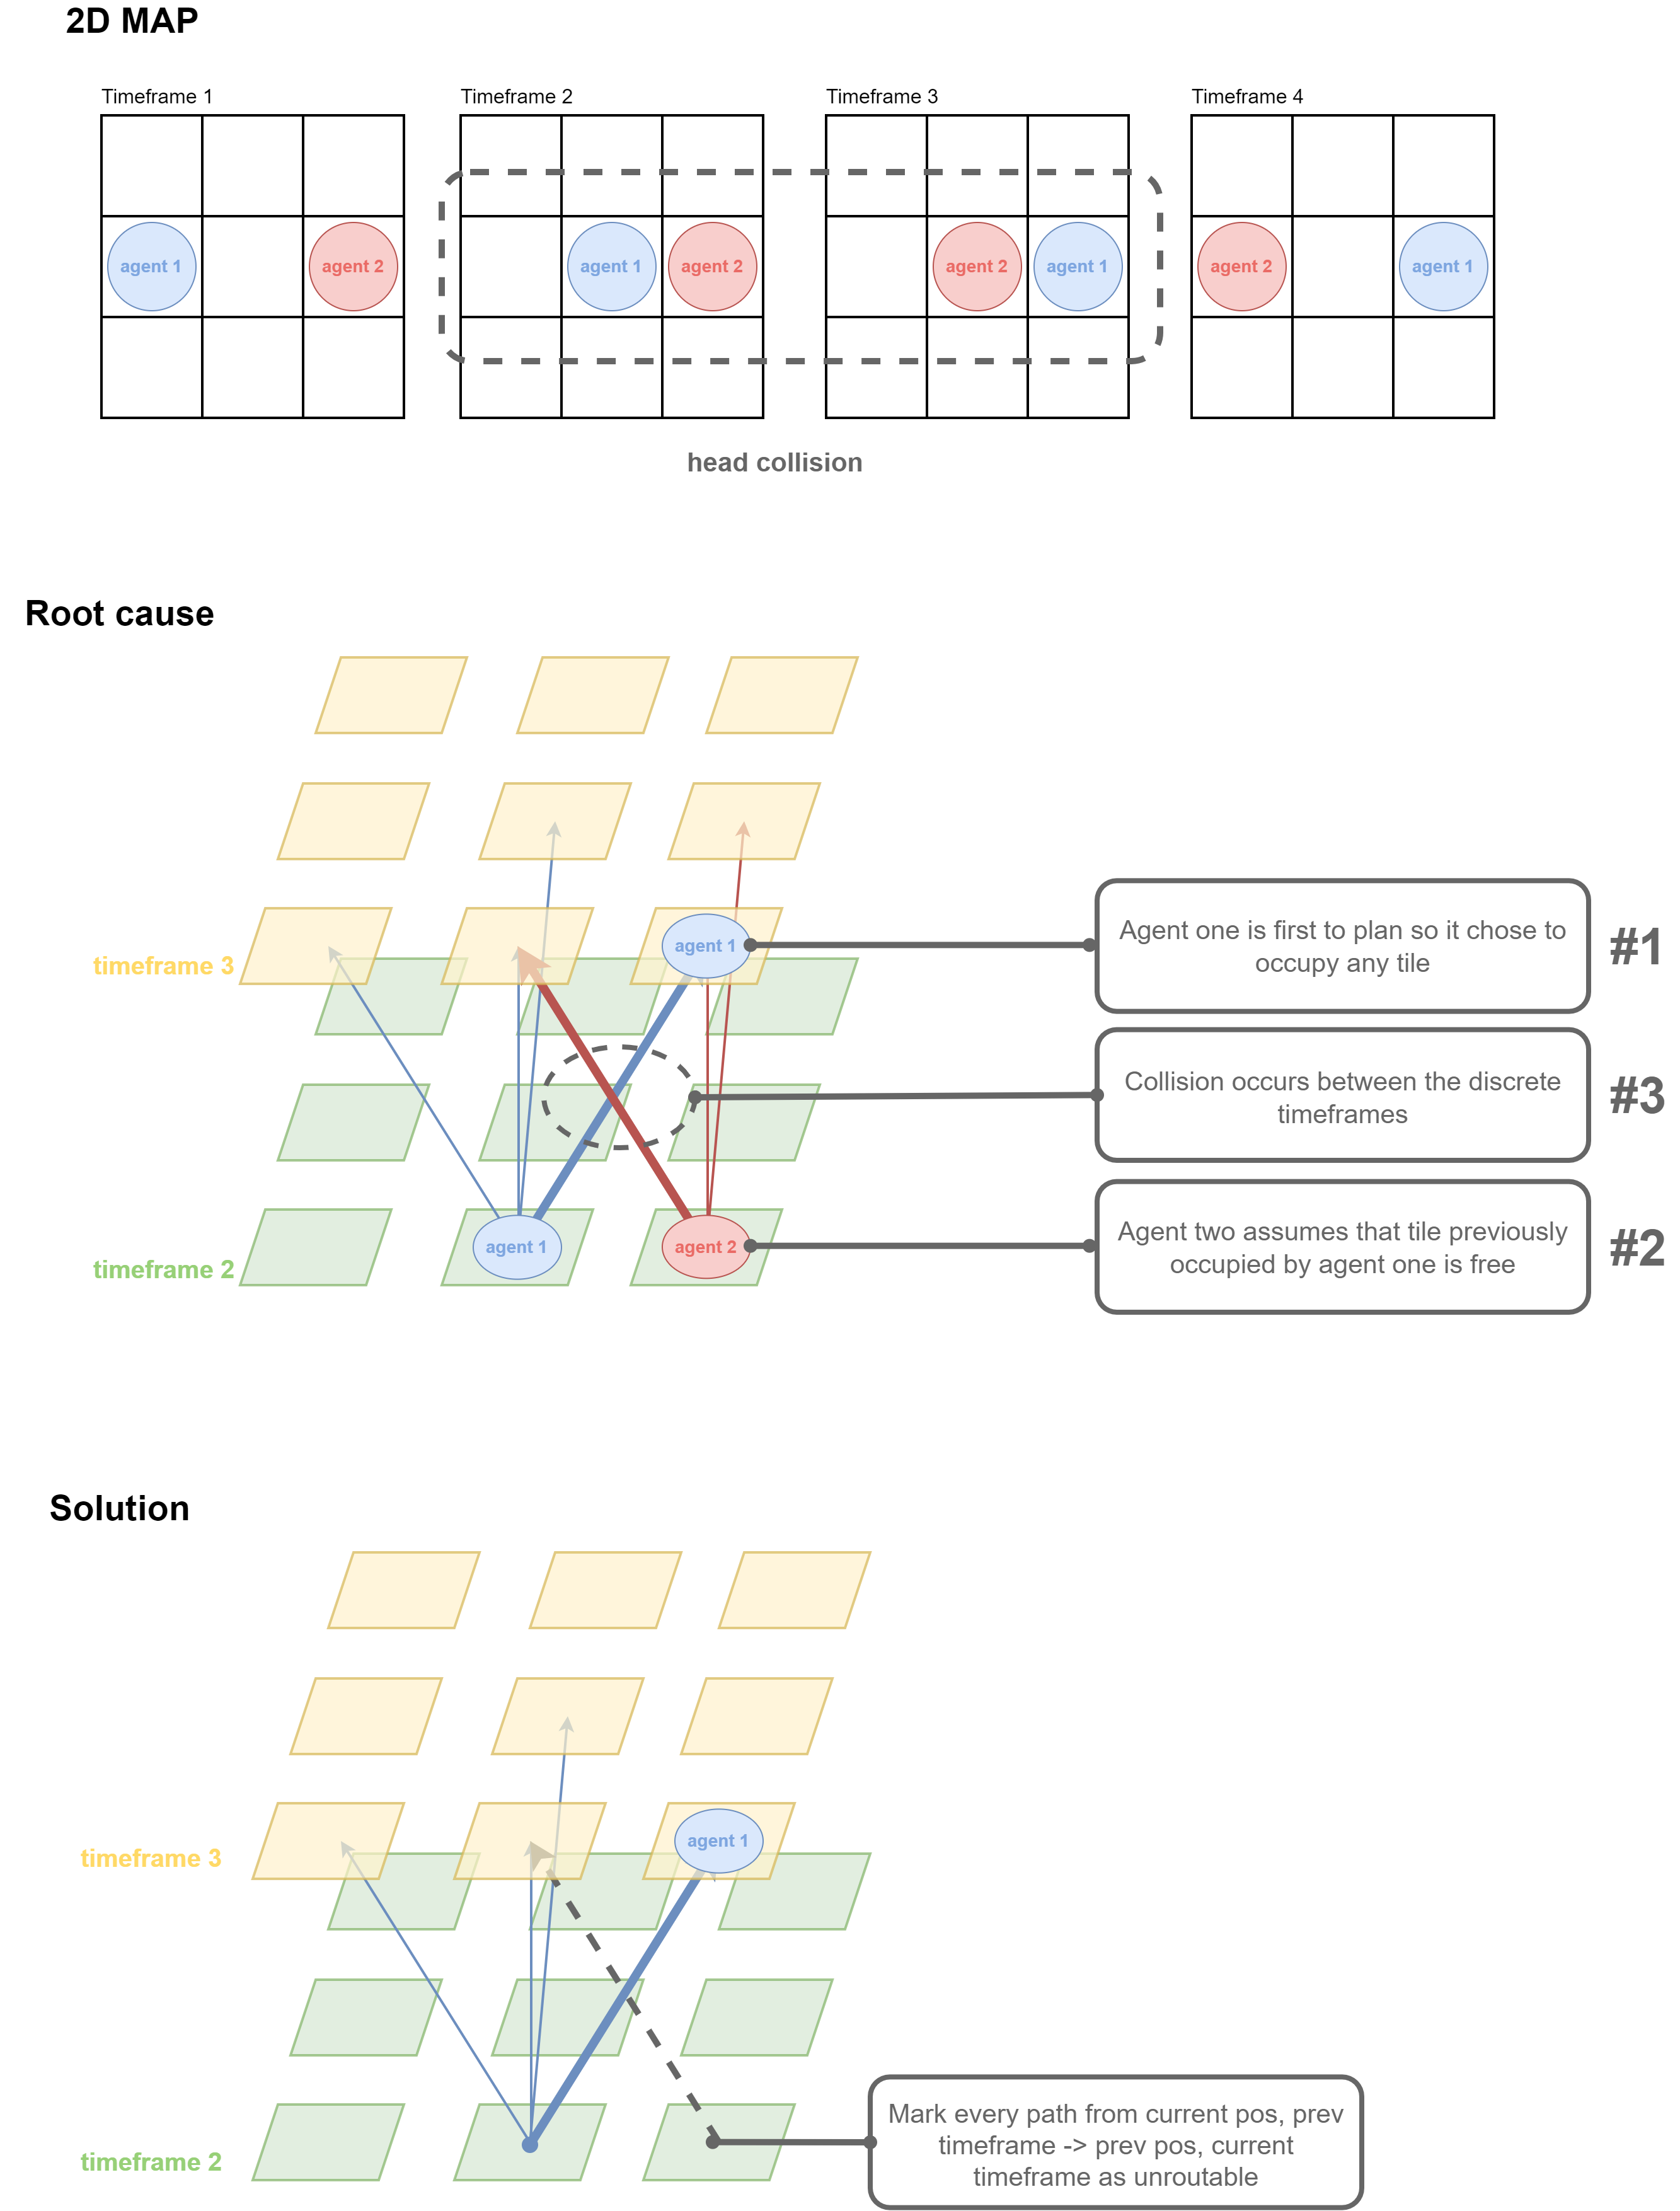
\includegraphics[width=0.7\textwidth]{pictures/head_collision_problem.png}
    \caption{ CA* head collision problem}
    \label{fig:head_collision}
\end{figure}